% The full network (Appendix C, next to the equations of sec:method:model), one
% figure for all three routers. The parts only some routers have are marked in
% the input and the readout. Layer shapes follow models/gnn_encoder.py and
% models/base_model.py. d is the width of a vertex embedding, 8 features before
% the first round and w after it. L and w are TBD (tab:modelparams), so they stay
% symbols here.
% Build:  latexmk -pdf architecture_detail.tex, then copy the pdf to Images/.
\documentclass[border=2pt]{standalone}
\usepackage{lmodern}
\usepackage[T1]{fontenc}
\usepackage{amsmath,amssymb}
\usepackage{tikz}
\usetikzlibrary{positioning,fit,backgrounds,arrows.meta,calc,decorations.pathreplacing}

% Palette shared with base.py (C dict).
\definecolor{storeF}{HTML}{CFE3F7}
\definecolor{taskF}{HTML}{F6E7C1}
\definecolor{ctrlF}{HTML}{D7F0D8}
\definecolor{estF}{HTML}{F7D6D6}
\definecolor{delF}{HTML}{FFD9B3}
\definecolor{commF}{HTML}{E8D9F0}
\definecolor{ink}{HTML}{43505C}
\definecolor{muted}{HTML}{5A6673}

\tikzset{
  layer/.style={draw=ink, line width=0.8pt, rounded corners=3pt, align=center,
                fill=white, text width=7.6cm, minimum height=0.95cm,
                inner sep=4pt, font=\small},
  side/.style={draw=ink, line width=0.8pt, rounded corners=3pt, align=center,
               text width=3.6cm, inner sep=4pt, font=\footnotesize},
  head/.style={draw=ink, line width=0.8pt, rounded corners=3pt, align=center,
               fill=ctrlF, text width=2.3cm, minimum height=1.6cm,
               inner sep=3pt, font=\footnotesize},
  flow/.style={-{Stealth[length=2.4mm]}, line width=0.9pt, draw=ink},
  opt/.style={flow, dashed},
  lbl/.style={font=\footnotesize, text=ink, align=center},
}

\begin{document}
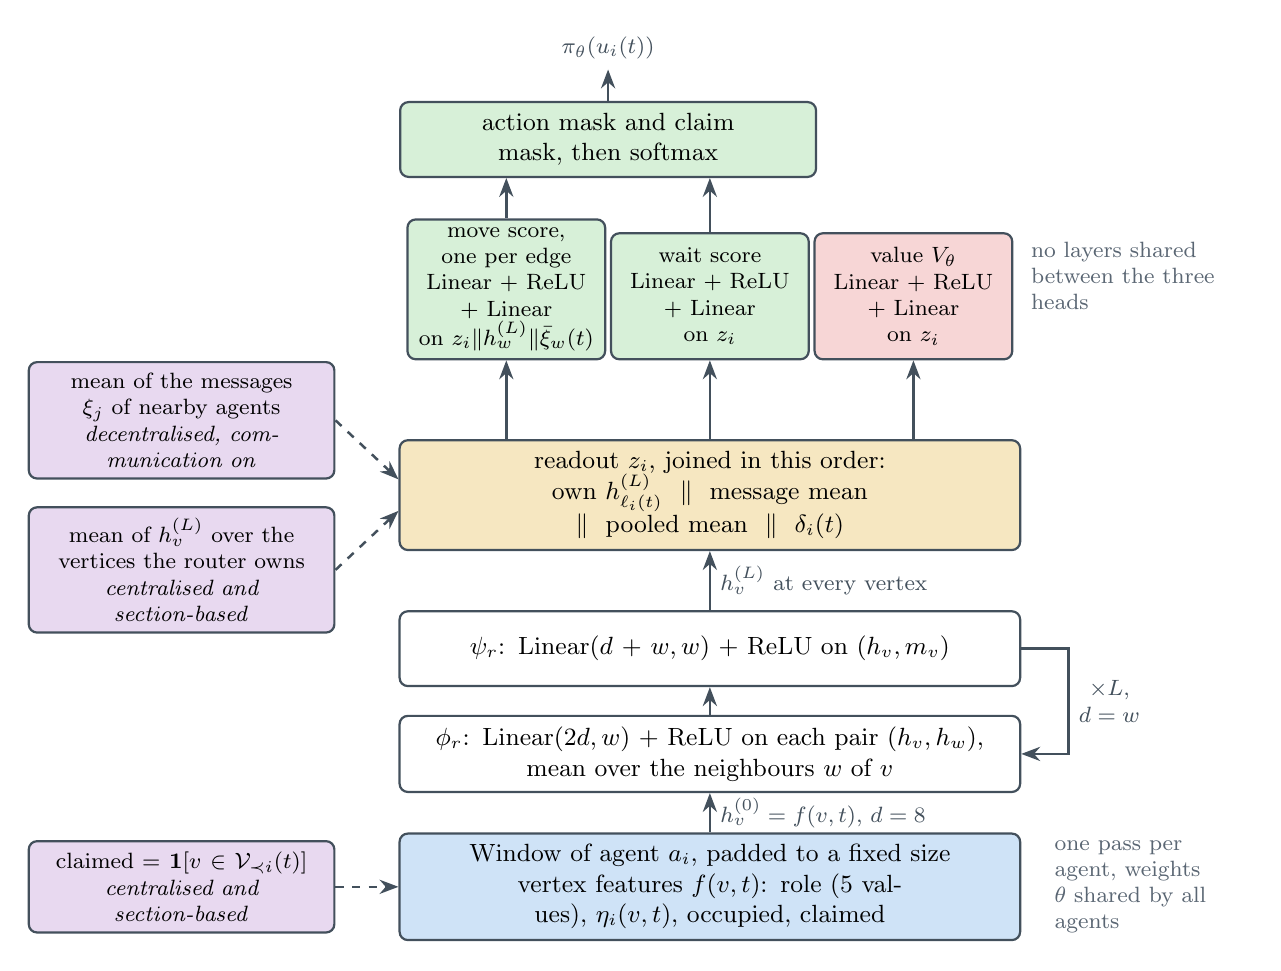
\begin{tikzpicture}
  % ---------------------------------------------------------- input
  \node[layer, fill=storeF] (in) {Window of agent $a_i$, padded to a fixed size\\
    vertex features $f(v,t)$: role (5 values), $\eta_i(v,t)$, occupied, claimed};
  \node[side, fill=commF, left=0.8cm of in] (claim)
    {claimed $= \mathbf{1}[v \in \mathcal{V}_{\prec i}(t)]$\\
    \textit{centralised and section-based}};
  \draw[opt] (claim) -- (in);

  % ---------------------------------------------------------- message passing
  \node[layer, above=0.5cm of in] (phi) {$\phi_r$: Linear$(2d, w)$ + ReLU on each pair $(h_v, h_w)$,\\
    mean over the neighbours $w$ of $v$};
  \node[layer, above=0.35cm of phi] (psi) {$\psi_r$: Linear$(d + w, w)$ + ReLU on $(h_v, m_v)$};
  \draw[flow] (in) -- node[right, lbl] {$h^{(0)}_v = f(v,t)$, $d = 8$} (phi);
  \draw[flow] (phi) -- (psi);
  \draw[flow] (psi.east) -- ++(0.6,0) |- node[pos=0.25, right, lbl] {$\times L$,\\ $d = w$} (phi.east);

  % ---------------------------------------------------------- readout
  \node[layer, above=0.75cm of psi, fill=taskF] (ro) {readout $z_i$, joined in this order:\\
    own $h^{(L)}_{\ell_i(t)}$ \ $\Vert$ \ message mean \ $\Vert$ \ pooled mean \ $\Vert$ \ $\delta_i(t)$};
  \draw[flow] (psi) -- node[right, lbl] {$h^{(L)}_v$ at every vertex} (ro);
  \node[side, fill=commF, left=0.8cm of ro, yshift=0.95cm] (msg)
    {mean of the messages $\xi_j$ of nearby agents\\
    \textit{decentralised, communication on}};
  \node[side, fill=commF, left=0.8cm of ro, yshift=-0.95cm] (pool)
    {mean of $h^{(L)}_v$ over the vertices the router owns\\
    \textit{centralised and section-based}};
  \draw[opt] (msg.east) -- ($(ro.west)+(0,0.2)$);
  \draw[opt] (pool.east) -- ($(ro.west)+(0,-0.2)$);

  % ---------------------------------------------------------- heads
  \node[head, above=1.0cm of ro.north west, anchor=south west, xshift=0.1cm] (score)
    {move score, one per edge\\ Linear + ReLU + Linear\\ on $z_i \Vert h^{(L)}_w \Vert \bar\xi_w(t)$};
  \node[head, above=1.0cm of ro.north, anchor=south] (wait)
    {wait score\\ Linear + ReLU + Linear\\ on $z_i$};
  \node[head, fill=estF, above=1.0cm of ro.north east, anchor=south east, xshift=-0.1cm] (V)
    {value $V_\theta$\\ Linear + ReLU + Linear\\ on $z_i$};
  \draw[flow] (ro.north -| score) -- (score);
  \draw[flow] (ro.north -| wait) -- (wait);
  \draw[flow] (ro.north -| V) -- (V);
  
  \node[layer, fill=ctrlF, text width=5.0cm, above=0.6cm of $(score.north)!0.5!(wait.north)$]
    (soft) {action mask and claim mask, then softmax};
  \draw[flow] (score.north) -- (score.north |- soft.south);
  \draw[flow] (wait.north) -- (wait.north |- soft.south);
  \draw[flow] (soft.north) -- ++(0,0.4) node[above, lbl] {$\pi_\theta(u_i(t))$};

  \node[lbl, text=muted, right=0.1cm of V.north east, anchor=north west, text width=2.4cm, align=left]
    {no layers shared between the three heads};
  \node[lbl, text=muted, right=0.3cm of in, text width=2.4cm, align=left]
    {one pass per agent, weights $\theta$ shared by all agents};
\end{tikzpicture}
\end{document}
